\documentclass{article}
\usepackage{tikz}
\usetikzlibrary{decorations.text}

\begin{document}

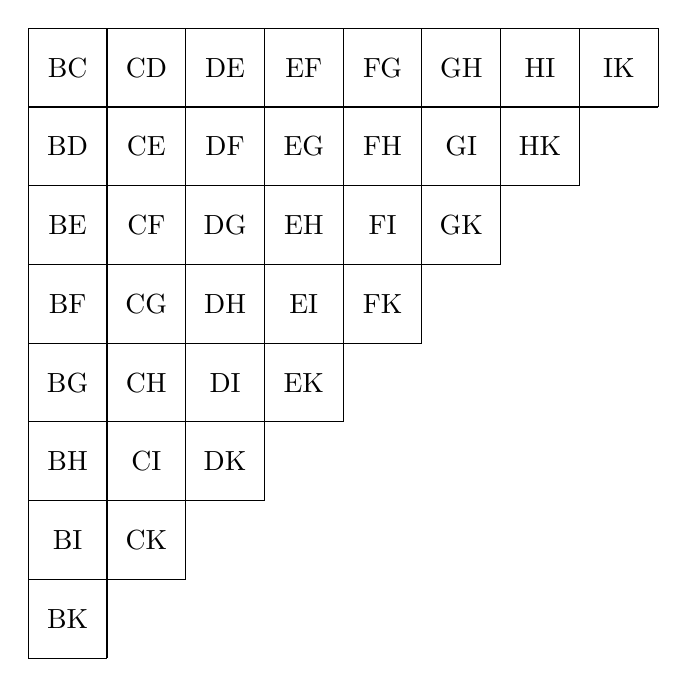
\begin{tikzpicture}

% Vertical
\draw (0,0) -- (0,-8);
\foreach \x in {1,...,8}
  \draw (\x,0) -- (\x,\x-9);

% Horizontal
\draw (0,0) -- (8,0);
\foreach \x in {1,...,8}
 \draw (0,-\x) -- (9-\x,-\x);

% Letters
\foreach \y in {0,...,7} {
  \pgfmathtruncatemacro{\maxx}{7-\y} % Classic TikZ Gotcha
  \foreach \x in {0,...,\maxx} {
    \pgfmathparse{{"B","C","D","E","F","G","H","I","K"}[\x]}
    \edef\initial{\pgfmathresult}
    \pgfmathparse{{"B","C","D","E","F","G","H","I","K"}[\y+1+\x]}
    \edef\final{\pgfmathresult}
    \draw (0.5+\x,-0.5-\y) node {\initial\final};
  }
}
\end{tikzpicture}

\end{document}
